% =====================================================================
%  Supplemental document for:
%  Estimates of Lunar Regolith Thermal Conductivity K_d at the
%  Apollo 15 and 17 Heat-Flow Boreholes.
%
%  Build: pdflatex appendix ; bibtex appendix ; pdflatex x2
%  Figures are produced by the repository pipeline:
%    fig_holdout.pdf            scripts/pipeline/retrieve_kd.py
%    fig_kd_qb_posterior.pdf    scripts/pipeline/bayesian_crosscheck.py
%    fig_posterior_compare.pdf  scripts/pipeline/bayesian_crosscheck.py
% =====================================================================
\documentclass[11pt]{article}

\usepackage[a4paper,margin=2.2cm]{geometry}
\usepackage[T1]{fontenc}
\usepackage{lmodern}
\usepackage{microtype}
\usepackage{amsmath,amssymb}
\usepackage{siunitx}
\sisetup{detect-all,per-mode=symbol}
\DeclareSIUnit{\year}{yr}
\usepackage{graphicx}
\usepackage{booktabs}
\usepackage{caption}
\captionsetup{font=small,labelfont=bf,labelsep=period}
\usepackage{xcolor}
\usepackage[hidelinks,colorlinks=true,linkcolor=blue!50!black,
            citecolor=blue!50!black,urlcolor=blue!60!black]{hyperref}
\usepackage[round,authoryear]{natbib}
\bibliographystyle{plainnat}

\renewcommand{\thesection}{S\arabic{section}}
\renewcommand{\thefigure}{S\arabic{figure}}
\renewcommand{\thetable}{S\arabic{table}}

\title{\bfseries Supporting Information for ``Estimates of Lunar Regolith
Thermal Conductivity $K_d$ at the Apollo 15 and 17 Heat-Flow Boreholes''}
\author{R.~P.~Gregorio et al.}
\date{\today}

\begin{document}
\maketitle

\noindent This supplement collects the held-out validation diagnostics
and the Bayesian $K_d$--$Q_b$ cross-check referenced in \S3.3 of the
main text. Every figure and number is regenerated by the public
repository (\url{https://github.com/rp3gregorio/Lunar-HFE}); the
generating script is named in each caption.

% =====================================================================
\section{Certification of the periodic-equilibrium solver}
\label{sec:s-solver}

The retrieval forward model computes the periodic steady state of the
flux-bottom-boundary column by the flux-anchored outer iteration
described in \S2.3 of the main text. Figure~\ref{fig:s-certification}
certifies its two defining properties at the retrieved per-site
$K_d^{*}$ values. \emph{(a) Initial-guess independence:} converged
cycle-mean profiles started from 240~K and 260~K agree to
$\le$19~mK at every depth in the 5-m column --- the initial thermal
state leaves no measurable imprint on the retrieval. \emph{(b)
Fixed-point drift:} a 120-lunation verification integration started
from the converged profile drifts by $\le$73~mK at the sensor depths,
bounding the residual solver systematic on $K_d^{*}$ at
$\lesssim$0.15~mW~m$^{-1}$~K$^{-1}$, an order of magnitude below the
bootstrap uncertainty. Both tests are regenerated by
\texttt{scripts/figures/make\_equilibrium\_certification.py}.

\begin{figure}[htbp]
\centering

\includegraphics[width=\linewidth]{figures/fig_equilibrium_certification.pdf}
\caption{Solver certification at the retrieved $K_d^{*}$.
\textbf{(a)} Absolute difference between converged cycle-mean profiles
from initial guesses of 240 and 260~K. \textbf{(b)} Absolute change of
the cycle-mean profile over a 120-lunation verification integration
started from the converged state. Shaded band: HFE sensor depths used
in the retrieval.}
\label{fig:s-certification}
\end{figure}

% =====================================================================
\section{Held-out validation of the per-site retrieval}
\label{sec:s-holdout}

Two internal checks confirm that the per-site $K_d^{*}$ retrieval is
not driven by a single sensor or sensor type. \emph{(i) TG vs.\ TR
cross-prediction:} fitting $K_d$ on the gradient-bridge (TG) sensors
alone and evaluating on the ring-bridge (TR) sensors, and vice versa.
\emph{(ii) Leave-one-deepest-out:} withholding the deepest sensor at
each site ($z=139$ cm at Apollo 15, $z=234$ cm at Apollo 17), refitting
$K_d$ on the remainder, and predicting the withheld temperature.
Results are summarised in Figure~\ref{fig:s-holdout}; the out-of-sample
degradations are quoted in the main text (\S3.3).

\begin{figure}[htbp]
\centering

\includegraphics[width=\linewidth]{figures/fig_holdout.pdf}
\caption{Held-out validation. \textbf{(a)} TG$\leftrightarrow$TR
cross-prediction RMSE (in-sample vs.\ out-of-sample) at both sites.
\textbf{(b)} Absolute residual at the withheld deepest sensor.
Generated by \texttt{scripts/pipeline/retrieve\_kd.py}.}
\label{fig:s-holdout}
\end{figure}

% =====================================================================
\section{Bayesian $K_d$--$Q_b$ cross-check}
\label{sec:s-bayes}

The non-parametric bootstrap is the primary uncertainty estimate in the
main text because it propagates only quantities measured at the
boreholes. As an independent check on the \emph{direction} of the
inter-site contrast, we also sample the joint posterior of $(K_d, Q_b)$
at each site with an affine-invariant MCMC ensemble sampler
\citep{foreman_mackey2013emcee}, placing the published basal-flux
envelopes \citep{langseth1976,saito2007,nagihara2018} as priors on
$Q_b$ and using the deep-sensor Gaussian likelihood built from the
cached RMSE($K_d$) curves. The posteriors trace the $K_d/Q_b$
degeneracy ridge discussed in \S4.2 of the main text; the marginal
medians differ from the bootstrap point estimates by construction (the
$Q_b$ prior slides each marginal along the ridge), but the ordering
$K_d^{\rm A17} > K_d^{\rm A15}$ is preserved with high posterior
probability (value quoted in \S3.3 of the main text).

\begin{figure}[htbp]
\centering
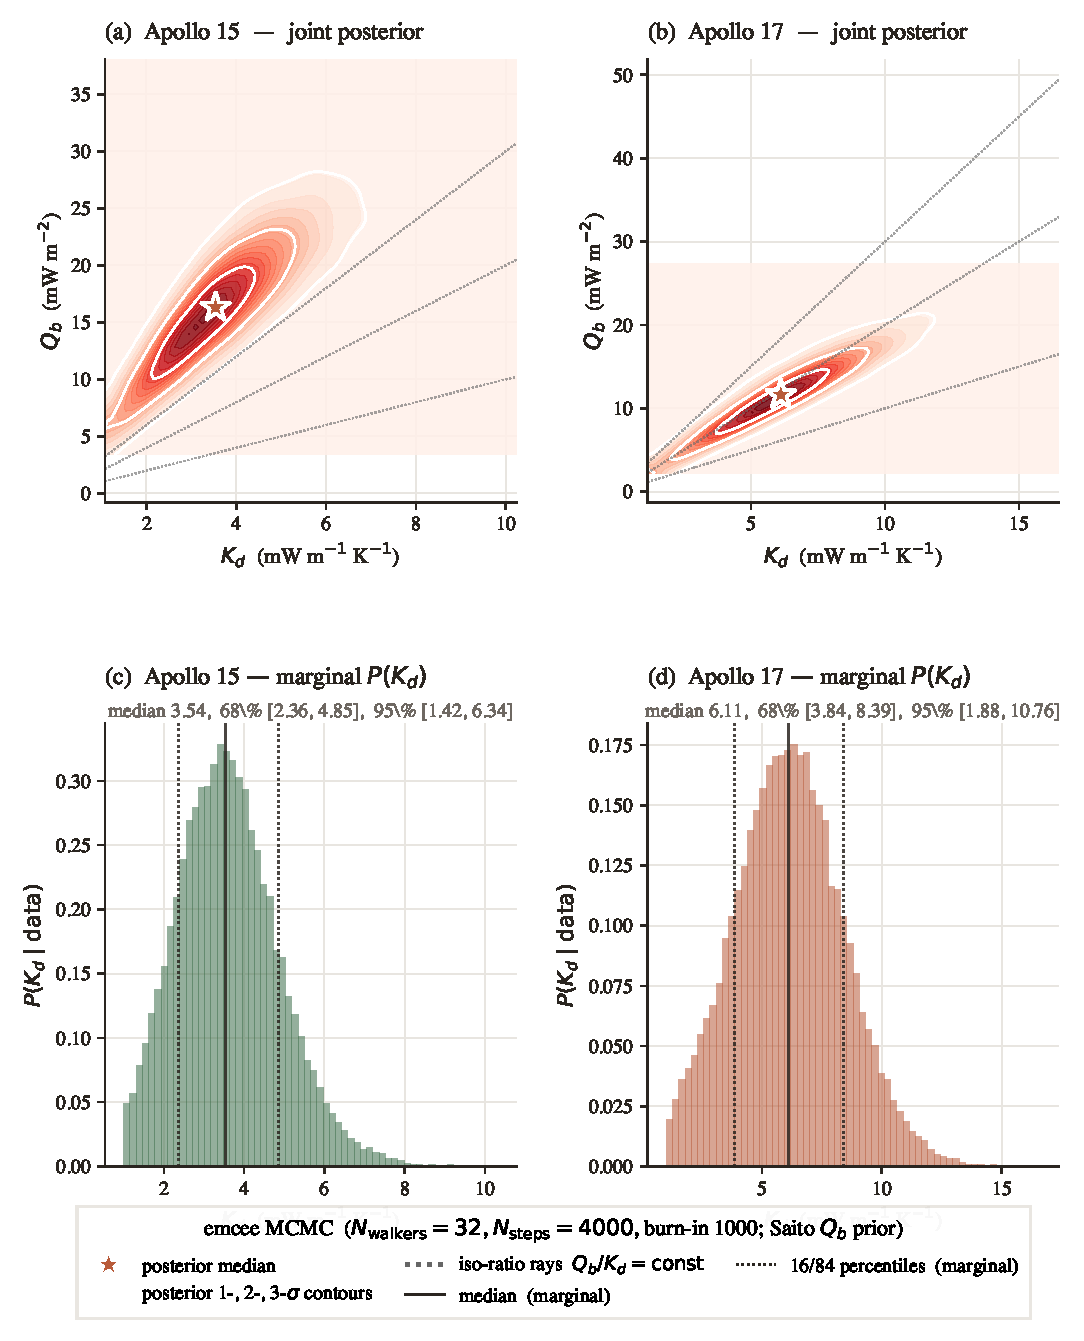
\includegraphics[width=\linewidth]{figures/fig_kd_qb_posterior.pdf}
\caption{Joint $(K_d, Q_b)$ posteriors at the two sites under the
published basal-flux priors. The diagonal elongation is the
$|\partial_z T| = Q_b/K_d$ degeneracy ridge. Generated by
\texttt{scripts/pipeline/bayesian\_crosscheck.py}.}
\label{fig:s-posterior}
\end{figure}

\begin{figure}[htbp]
\centering
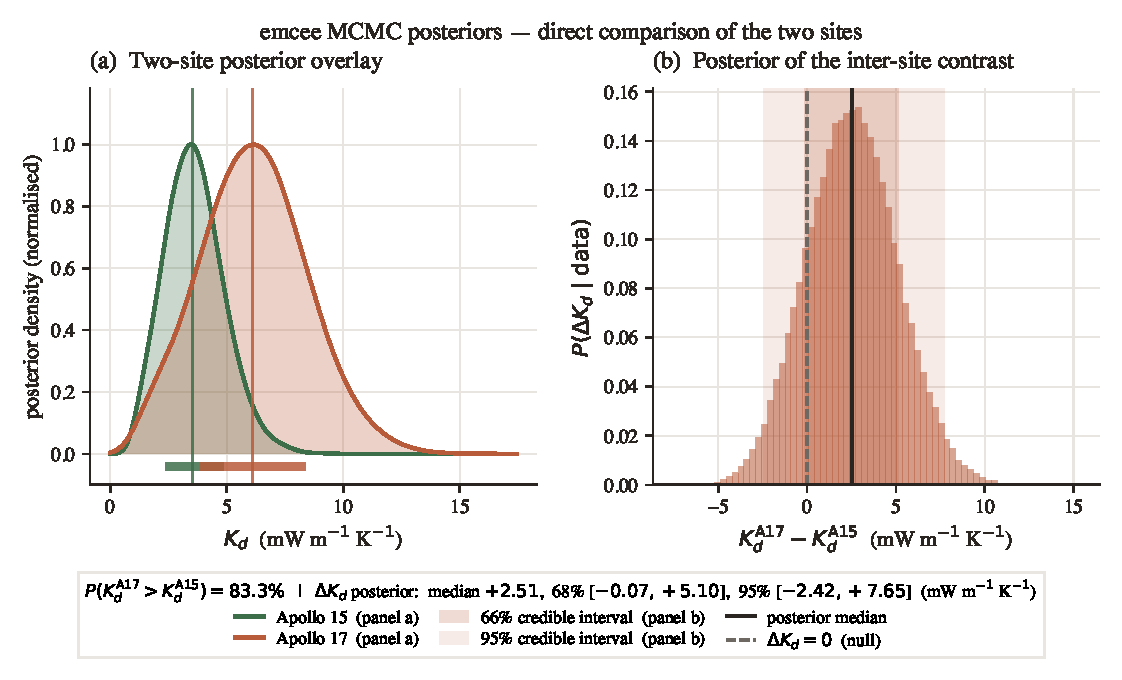
\includegraphics[width=\linewidth]{figures/fig_posterior_compare.pdf}
\caption{Marginal $K_d$ posteriors compared with the bootstrap
distributions of the main text (Fig.~4). Generated by
\texttt{scripts/pipeline/bayesian\_crosscheck.py}.}
\label{fig:s-compare}
\end{figure}

\bibliography{../letter/references}

\end{document}
